\documentclass[aspectratio=169,10pt]{beamer}
\usetheme{default}
\usecolortheme{default}
\usefonttheme{professionalfonts}
\setbeamertemplate{navigation symbols}{}
\setbeamertemplate{footline}{\hfill\insertframenumber\,/\,\inserttotalframenumber\hspace{1em}\vspace{0.7em}}
\setbeamercolor{structure}{fg=blue!55!black}
\usepackage[T1]{fontenc}
\usepackage[utf8]{inputenc}
\usepackage[ngerman]{babel}
\usepackage{amsmath}
\usepackage{booktabs}
\usepackage{graphicx}
\usepackage{tabularx}
\graphicspath{{../results/run_20261108_143652/}{../results/run_20261109_093542/}}

\title{Neuronale Ersatzmodelle für Biegelinien}
\subtitle{Analytische Studie und Weg zum FEM-basierten Modell}
\author{Mirco Buck \and Daniel Dietzsch}
\institute{Universität Ulm}
\date{10. November 2026}
\newcommand{\singleplot}[1]{\includegraphics[width=.96\linewidth,height=.72\textheight,keepaspectratio]{#1}}

\begin{document}
\begin{frame}\titlepage\end{frame}

\begin{frame}{Zielsetzung}
\begin{itemize}
  \item Biegelinien sollen durch ein neuronales Ersatzmodell schnell vorhergesagt werden.
  \item Die analytische Studie trennt den Einfluss von Netzarchitektur, Datenmenge und Geometrie.
  \item Anschließend soll dieselbe Idee auf FEM-Daten übertragen werden.
\end{itemize}
\vfill
Leitfrage: Wann liefert ein datengetriebenes Modell zuverlässige Interpolation und wann versagt es außerhalb des Trainingsbereichs?
\end{frame}

\begin{frame}{Neuronales Netz: Eingabe und Ausgabe}
\begin{columns}[T]
\column{.47\textwidth}
\textbf{Eingabe}
\[
\boldsymbol{z}=\left[x/L,\; L,\; F,\; a/L,\; h_2/h_1\right]
\]
Je nach Balkenmodell entfallen die letzten beiden Größen. Die Eingabe beschreibt Position, Last und Geometrie.
\column{.47\textwidth}
\textbf{Ausgabe}
\[
\widehat w(\boldsymbol{z})
\]
Das Netz schätzt die Durchbiegung an der angegebenen Position. Für einen ganzen Balken wird die Abfrage für viele Positionen wiederholt.
\end{columns}
\vfill
Ein Ersatzmodell ersetzt nicht die Physik. Es lernt die Zuordnung von Eingabegrößen zu Referenzlösungen.
\end{frame}

\begin{frame}{Mehrschichtiges Perzeptron}
\begin{columns}[T]
\column{.52\textwidth}
Eine Schicht berechnet gewichtete Summen und wendet eine Aktivierungsfunktion an:
\[
\boldsymbol{h}=\tanh\!\left(W\boldsymbol{z}+\boldsymbol{b}\right).
\]
Mehrere versteckte Schichten können nichtlineare Zusammenhänge abbilden. Die letzte Schicht ist hier linear, damit die Durchbiegung jeden Wert annehmen kann.
\column{.42\textwidth}
\begin{center}\fbox{\parbox{.82\linewidth}{\centering
Eingabevektor\\[0.6em] $\downarrow$\\[0.6em]
versteckte Tanh-Schicht(en)\\[0.6em] $\downarrow$\\[0.6em]
lineare Ausgabeschicht\\[0.6em] $\downarrow$\\[0.6em]
Durchbiegung $\widehat w$}}
\end{center}
\end{columns}
\end{frame}

\begin{frame}{Training eines neuronalen Netzes}
\begin{enumerate}
  \item Referenzdaten liefern Paare aus Eingabe $\boldsymbol{z}_i$ und Durchbiegung $w_i$.
  \item Das Netz berechnet eine Vorhersage $\widehat w_i$.
  \item Der mittlere quadratische Fehler bewertet die Abweichung:
  \[
  \mathcal{L}=\frac{1}{N}\sum_{i=1}^{N}\left(\widehat w_i-w_i\right)^2.
  \]
  \item Ein Optimierer verändert Gewichte und Biases, bis der Fehler klein wird.
\end{enumerate}
\vfill In dieser Studie: Tanh-Aktivierung, linearer Ausgang und L-BFGS-Optimierung.
\end{frame}

\begin{frame}{Datenaufteilung und faire Bewertung}
\begin{columns}[T]
\column{.49\textwidth}
\textbf{Training und Validierung}
\begin{itemize}
  \item 80 oder 160 Balkenfälle zum Training
  \item Validierungsfälle wählen Architektur und Seed
  \item fünf zufällige Initialisierungen je Architektur
\end{itemize}
\column{.49\textwidth}
\textbf{Unabhängige Tests}
\begin{itemize}
  \item Interpolation: neue Fälle innerhalb des bekannten Bereichs
  \item Extrapolation: Last, Länge und beim Sprung auch Geometrie außerhalb des Bereichs
  \item Fehlermaß: $e_{\max}=\max_x\frac{|\widehat w(x)-w(x)|}{|w(L)|}$
\end{itemize}
\end{columns}
\end{frame}

\begin{frame}{Vorgehensweise}
\begin{enumerate}
  \item \textbf{Analytischer MLP:} Biegelinien aus bekannten Formeln erzeugen und die Lernbarkeit systematisch untersuchen.
  \item \textbf{FEM-Datensatz:} Parameterisierte FEM-Rechnungen erzeugen Verformungsfelder für realistischere Geometrien und Randbedingungen.
  \item \textbf{Drei Ersatzmodelle vergleichen:} POD-MLP, PINN und direkter MLP auf den FEM-Daten.
\end{enumerate}
\vfill Die folgenden Ergebnisfolien betreffen ausschließlich Schritt 1. Die FEM-Methoden sind der geplante nächste Abschnitt.
\end{frame}

\begin{frame}{Analytische Referenzmodelle}
\begin{columns}[T]
\column{.48\textwidth}\textbf{Konstanter Querschnitt}
\[w(x)=\frac{F x^2(3L-x)}{6EI}\]
$E=210\,\mathrm{GPa}$, \quad $I=8{,}333\cdot10^{-6}\,\mathrm{m}^4$
\column{.48\textwidth}\textbf{Querschnittssprung}
\begin{itemize}
  \item Sprungstelle $a/L\in[0{,}2,0{,}8]$
  \item Höhenverhältnis $h_2/h_1\in[0{,}6,1{,}5]$
  \item $I_2=I_1(h_2/h_1)^3$
\end{itemize}
Die Durchbiegung und Neigung bleiben an $x=a$ stetig. Die Krümmung ändert sich abschnittsweise.
\end{columns}
\end{frame}

\begin{frame}{Studienaufbau der analytischen Untersuchung}
\centering
\begin{tabular}{lll}\toprule
Geometrie & Netzarchitektur & Trainingsfälle\\ \midrule
Konstanter Querschnitt & 1 Layer, 1 bis 15 Neuronen & 80 und 160\\
Konstanter Querschnitt & 2 Layer, 56 Kombinationen & 80 und 160\\
Querschnittssprung & 1 Layer, 1 bis 15 Neuronen & 80 und 160\\
Querschnittssprung & 2 Layer, 56 Kombinationen & 80 und 160\\ \bottomrule
\end{tabular}
\vfill Insgesamt wurden 1.420 Trainingsläufe durchgeführt.
\end{frame}

\begin{frame}{Konstanter Querschnitt: ein Layer, 80 Fälle}\centering\singleplot{constant_1layer_80cases/main_plot.png}\end{frame}
\begin{frame}{Konstanter Querschnitt: ein Layer, 160 Fälle}\centering\singleplot{constant_1layer_160cases/main_plot.png}\end{frame}
\begin{frame}{Konstanter Querschnitt: zwei Layer, 80 Fälle}\centering\singleplot{constant_2layer_80cases/main_plot.png}\end{frame}
\begin{frame}{Konstanter Querschnitt: zwei Layer, 160 Fälle}\centering\singleplot{constant_2layer_160cases/main_plot.png}\end{frame}

\begin{frame}{Ergebnisse des konstanten Balkens}
\centering\begin{tabular}{lrrr}\toprule
Netz und Fälle & Architektur & Interpolation & Extrapolation\\ \midrule
1 Layer, 80 & 15 & 0,30\% & 5,32\%\\
1 Layer, 160 & 15 & 0,18\% & 5,94\%\\
2 Layer, 80 & [8 5] & 0,33\% & 5,00\%\\
2 Layer, 160 & [8 5] & 0,32\% & 6,40\%\\ \bottomrule
\end{tabular}
\vfill\begin{itemize}
\item 160 Fälle verbessern die Interpolation beim einfachen Netz.
\item Zwei Layer helfen nicht, obwohl sie mehr Parameter besitzen.
\item Die Extrapolation bleibt deutlich unsicherer als die Interpolation.
\end{itemize}
\end{frame}

\begin{frame}{Querschnittssprung: ein Layer, 80 Fälle}\centering\singleplot{step_1layer_80cases/main_plot.png}\end{frame}
\begin{frame}{Querschnittssprung: ein Layer, 160 Fälle}\centering\singleplot{step_1layer_160cases/main_plot.png}\end{frame}
\begin{frame}{Querschnittssprung: zwei Layer, 80 Fälle}\centering\singleplot{step_2layer_80cases/main_plot.png}\end{frame}
\begin{frame}{Querschnittssprung: zwei Layer, 160 Fälle}\centering\singleplot{step_2layer_160cases/main_plot.png}\end{frame}

\begin{frame}{Architekturlandschaft beim Sprungmodell}
\centering\singleplot{step_2layer_160cases/architecture_heatmaps.png}
\vfill Sehr kleine erste Schichten sind ungeeignet. Eine größere erste Schicht senkt den Fehler, beseitigt aber die Extrapolationsgrenze nicht.
\end{frame}

\begin{frame}{Ergebnisse des Sprungmodells}
\centering\begin{tabular}{lrrr}\toprule
Netz und Fälle & Architektur & Interpolation & Extrapolation\\ \midrule
1 Layer, 80 & 14 & 29,65\% & 85,54\%\\
1 Layer, 160 & 14 & 10,58\% & 85,17\%\\
2 Layer, 80 & [8 6] & 13,24\% & 84,47\%\\
2 Layer, 160 & [7 6] & 8,43\% & 81,14\%\\ \bottomrule
\end{tabular}
\vfill\begin{itemize}
\item Mehr Daten und zwei Schichten verbessern die Interpolation deutlich.
\item Das 1-\%-Ziel wird beim Sprungmodell noch nicht erreicht.
\item Die Extrapolation bleibt in allen Varianten unzuverlässig.
\end{itemize}
\end{frame}

\begin{frame}{Grenze der Extrapolation}
\centering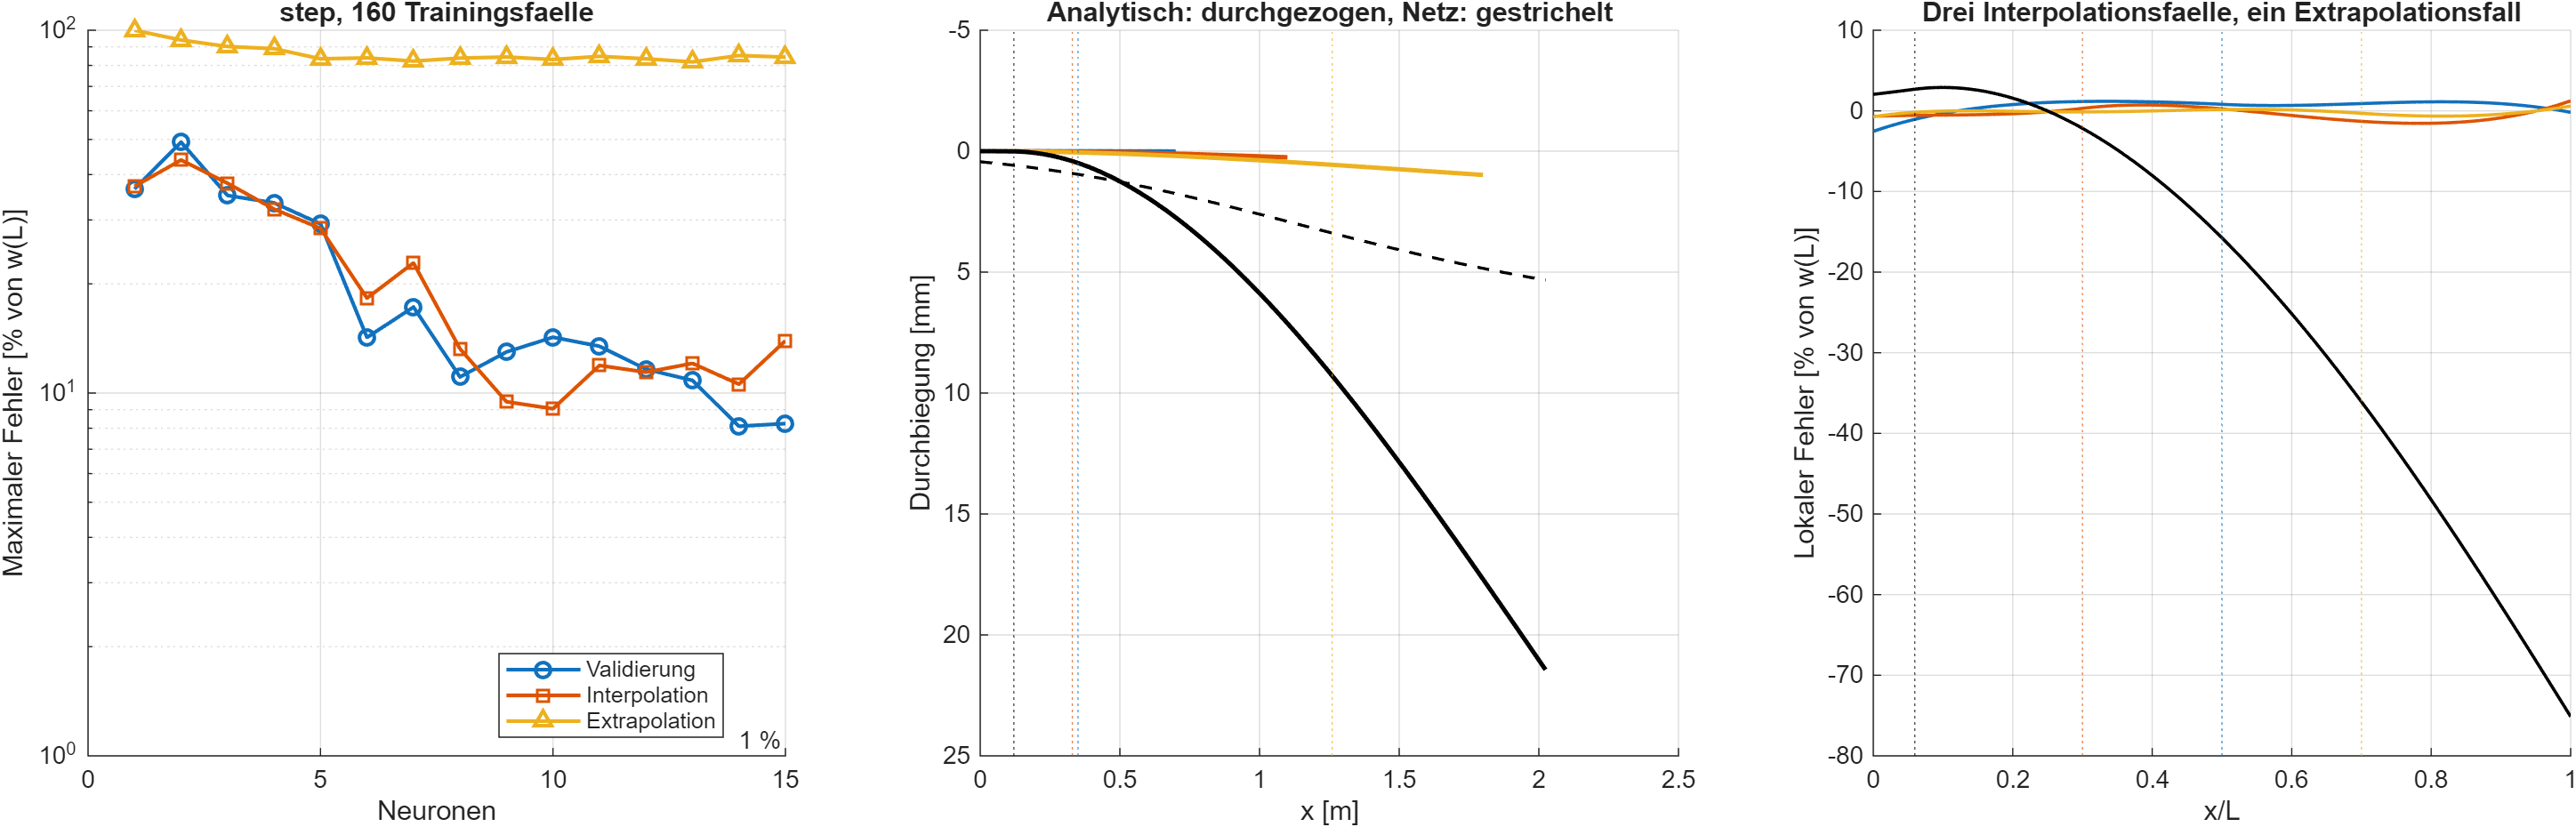
\includegraphics[width=.94\linewidth,height=.48\textheight,keepaspectratio]{step_1layer_160cases/main_plot.png}
\vfill
Im Extrapolationsfall wächst die analytische Durchbiegung stark. Die Netzvorhersage bleibt dagegen nahe einer flachen Kurve. Die Tanh-Schicht sättigt außerhalb des bekannten Eingabebereichs. Das erklärt die hohen Extrapolationsfehler von etwa 81 bis 86\% beim Sprungmodell.
\end{frame}

\begin{frame}{Erkenntnisse aus der analytischen Studie}
\begin{itemize}
\item Der glatte, konstante Balken lässt sich im bekannten Bereich sehr genau approximieren.
\item Ein Querschnittssprung erhöht die Schwierigkeit deutlich.
\item Die Validierung wählt ein Modell aus, garantiert aber keine robuste Extrapolation.
\item Sinnvolle Verbesserungen sind normierte Eingaben, die relative Distanz zur Sprungstelle und mehr Daten in deren Umgebung.
\end{itemize}
\end{frame}

\begin{frame}{FEM-Datensatz: geplanter nächster Schritt}
\begin{itemize}
\item Parameterisierte FEM-Rechnungen variieren Geometrie, Material, Last und Randbedingungen.
\item Jede Rechnung liefert ein räumliches Verformungsfeld statt nur einer analytischen Biegelinie.
\item Einheitliche Netze, Koordinaten und Skalierungen machen die Fälle vergleichbar.
\item Getrennte Parameterbereiche prüfen wieder Interpolation und Extrapolation.
\end{itemize}
\vfill\textbf{Status:} Konzept für die weiterführende Untersuchung. FEM-Ergebnisse liegen in diesem Vortrag noch nicht vor.
\end{frame}

\begin{frame}{POD-MLP: reduzierte FEM-Felder}
\begin{columns}[T]
\column{.55\textwidth}Die Proper Orthogonal Decomposition (POD) zerlegt viele FEM-Verformungsfelder in räumliche Basisfelder und wenige Koeffizienten:
\[\boldsymbol{u}\approx\overline{\boldsymbol{u}}+\Phi\boldsymbol{c}.\]
Ein MLP lernt dann nur die Abbildung von Parametern auf die Koeffizienten $\boldsymbol{c}$.
\column{.38\textwidth}\begin{center}\fbox{\parbox{.82\linewidth}{\centering FEM-Felder\\[0.4em] $\downarrow$ POD\\[0.4em] Basis $\Phi$ und Koeffizienten $\boldsymbol{c}$\\[0.4em] $\downarrow$ MLP\\[0.4em] vorhergesagtes Feld}}\end{center}
\end{columns}
\vfill Vorteil: Das Netz lernt einen kompakten Zielvektor statt aller Knotenwerte.
\end{frame}

\begin{frame}{PINN: Physik in der Verlustfunktion}
Ein Physics-Informed Neural Network gibt ein Feld $\widehat{\boldsymbol{u}}(\boldsymbol{x})$ aus. Neben Datenfehlern bestraft das Training Verletzungen der physikalischen Gleichungen und Randbedingungen:
\[\mathcal{L}=\mathcal{L}_{\mathrm{Daten}}+\lambda_{\mathrm{PDE}}\mathcal{L}_{\mathrm{PDE}}+\lambda_{\mathrm{RB}}\mathcal{L}_{\mathrm{RB}}.\]
\begin{itemize}
\item Die Modellgleichung liefert zusätzliche Information zwischen den Stützstellen.
\item Randbedingungen werden direkt im Trainingsziel berücksichtigt.
\item Die Gewichtung der Verlustanteile und die Trainingsstabilität müssen untersucht werden.
\end{itemize}
\vfill\textbf{Status:} geplanter Vergleichsansatz für den FEM-Datensatz.
\end{frame}

\begin{frame}{Direkter MLP auf FEM-Daten}
\begin{columns}[T]
\column{.5\textwidth}Eingabe: Geometrie-, Material- und Lastparameter sowie räumliche Koordinaten.

Ausgabe: Verschiebungskomponenten oder Spannungen an dieser Koordinate.

Das Vorgehen entspricht der analytischen Studie, nur die Referenzlösung stammt aus der FEM.
\column{.43\textwidth}\begin{center}\fbox{\parbox{.85\linewidth}{\centering Parameter und Koordinate\\[0.5em] $\downarrow$\\[0.5em] direkter MLP\\[0.5em] $\downarrow$\\[0.5em] Feldwert an der Koordinate}}\end{center}
\end{columns}
\vfill Dieser Ansatz dient als direkte Referenz für POD-MLP und PINN.
\end{frame}

\begin{frame}{Vergleich der weiterführenden Modelle}
\centering\begin{tabular}{p{.22\linewidth}p{.31\linewidth}p{.33\linewidth}}\toprule
Modell & Zielgröße & zentrale Prüffrage\\ \midrule
Direkter MLP & Feldwert an einer Koordinate & Reicht ein reines Datenmodell aus?\\
POD-MLP & wenige POD-Koeffizienten & Wie viel Genauigkeit bleibt nach der Reduktion?\\
PINN & kontinuierliches Feld & Verbessert die Physik die Generalisierung?\\ \bottomrule
\end{tabular}
\vfill Für alle drei Ansätze gelten dieselben Testbereiche und normierten Fehlermetriken.
\end{frame}

\begin{frame}{Fazit und nächste Schritte}
\begin{itemize}
\item Die analytische Studie etabliert eine belastbare Referenz für Datenmenge, Architektur und Testaufteilung.
\item Interpolation funktioniert beim einfachen Balken sehr gut, beim Sprung nur eingeschränkt.
\item Extrapolation bleibt die entscheidende Schwachstelle der rein datengetriebenen Modelle.
\item Als Nächstes folgen FEM-Datensatz, POD-MLP, PINN und direkter MLP im gleichen Bewertungsrahmen.
\end{itemize}
\end{frame}
\end{document}
